\documentclass{article}
\usepackage[labelfont={bf}]{caption}
\usepackage{booktabs,lipsum}
\usepackage{makecell}
\usepackage{multirow}
\usepackage[letterpaper, landscape, margin=2in]{geometry}
\usepackage{booktabs,caption,fixltx2e}
\usepackage[flushleft]{threeparttable}
\usepackage{caption}
\usepackage{bm}
\usepackage{tikz}
\usetikzlibrary{snakes}

\begin{document}


% & \thead{\# Obs.} &  \thead{Avg \# Obs/day} & Source\\
\begin{table}
\begin{threeparttable}
\caption{Data Descriptions}
\begin{tabular}{ |p{6cm}||p{2cm}|p{3cm}|p{6cm}|  }
 \hline
 \hline
 & \# Obs. &  Avg \# Obs/day & Source\\
 \hline
 Crimes - Theft                      & 215,075    & 425     & Chicago Police Department \\
 Crimes - Non-Theft                  & 128,487    & 253     & \\
 \hline
 Building Violations                 & 165,681    & 324     & Chicago Department of Buildings\\
 \hline
 311 Graffiti Request                & 164,318    & 321     & City of Chicago 311 Requests \\
 311 Sanitation Request              & 28,537     & 55      & \\
 311 Alley Lights Out                 & 44,166      & 86       & \\
 311 Vacant Building - Gangs         & 2,243      & 4       & \\
 311 Vacant Building Out - No Gangs  & 4,333      & 8       & \\
 \hline
 Food Inspection - Pass              & 16,945     & 33 & \multirow{3}{4cm}{Chicago Department of Public Helath Food Protection Program} \\ 
 Food Inspection - Pass w/Condition  & 5,674      & 11 & \\ 
 Food Inspection - Fail              & 3,342      & 6  & \\ 
 \hline
 Red Light Tickets\textsuperscript{1}                   & 86,817     & 964     & Chicago Tribune\\
 \hline
 Liquor Licenses\textsuperscript{2}                     & 4,541      & n/a     & Department of Business Affairs and Consumer Protection, City of Chicago\\
 \hline
 Tweets - Good Sentiment\textsuperscript{3}          & 1,052        & n/a     & Twitter\\
 Tweets - Bad Sentiment                & 183         & n/a      & \\
 \hline
\end{tabular}
\begin{tablenotes}
      \small
      \item 1. Red light ticket data is only available from 12/2/2013 to 1/3/2014 \\
          2. Liquor Licenses dataset is for current liscenses only so it is not shown over time. \\
          3. Twitter dataset was added recently so there is no historical data past what was collected.
    \end{tablenotes}
    \end{threeparttable}
\end{table}
\clearpage
\begin{table}
\begin{threeparttable}
\caption{311 Descriptions}
\begin{tabular}{ |p{6cm}||p{10cm}|  }
 \hline
 \hline
 & Description\\
  \hline
 311 Graffiti Request                & Requests to remove graffiti with city “blast” trucks    \\
 \hline
 311 Sanitation Request              & Complaints such as overflowing dumpsters or garbage in the Alley     \\
 \hline
 311 Alley Lights Out - Gangs        & One or more street lights out with reported Gangs or Homeless      \\
 \hline
 311 Alley Lights Out - No Gangs     & One or more street lights out without reported Gangs or Homeless      \\
 \hline
 311 Vacant Building  & Requests to inspect a vacant building      \\

  \hline
\end{tabular}

    \end{threeparttable}
\end{table}
\clearpage
\begin{table}
\begin{threeparttable}
\caption{Food Inspection Descriptions}
\begin{tabular}{ |p{4cm}||p{12cm}|  }
 \hline
 \hline
 & Description\\
  \hline
 Pass                & The establishment meets the minimum requirements of municipal codes and does not have any serious or critical violations 
    \\
 \hline
 Pass with Conditions              & The establishment has Serious or Critical violations that are corrected during the inspection or the certified Food Service Sanitation Manager is not present as the time of the Inspection     \\
 \hline
 Fail        & The establishment has Serious violations that cannot be corrected during the inspection. The business must correct the Serious violations promptly and pass a re- inspection to remain open. Note: the business can also have its license suspended until it passes re-inspection.       \\


  \hline
\end{tabular}

    \end{threeparttable}
\end{table}
\clearpage



\begin{table}
\begin{threeparttable}
\caption{Tweet Examples}
\begin{tabular}{ |p{1cm}|p{2cm}||p{12cm}|  }
 \hline
 \hline
Score & Category & Tweet\\
  \hline
 .55      &    Good      & I love this place already! - Drinking a Slim Hazy by @mikerphonebrew at @mikerphonebrew  — https://t.co/8EdB6ERhfJ
    \\
 \hline
 .72   &     Good      & Here's our Morton Community who supported our fundraiser event today! THANK YOU all who could not make it but con… https://t.co/rKrqMPWf7u    \\
 \hline
 -.36   &   Bad  & I'm really not trying to be in the crib tonight        \\
 \hline
 -.35   &   Bad  & Muffler: \$160 Battery: \$150 Alternator: \$350  Me: Broke as ****        \\
  \hline
\end{tabular}

    \end{threeparttable}
\end{table}
\clearpage



\begin{figure}
\centering
OLS Regression
\[ Theft_{(t,j)} = \alpha + \beta_1 \bm{X}_{(t,j)} + \beta_2 \bm{X}_{j} + \epsilon_t \]
Spatial OLS Regression\\ 
\[ Theft_{(t,j)} = \alpha + \beta_1 \bm{X}_{(t,j)} + \beta_2 \bm{X}_j + \beta_3 \bm{\bar{X}}_{(t,{j_{neighbors}})} + \beta_4 \bm{\bar{X}}_{(j_{neighbors})} + \epsilon_t \]
\end{figure}


\clearpage

  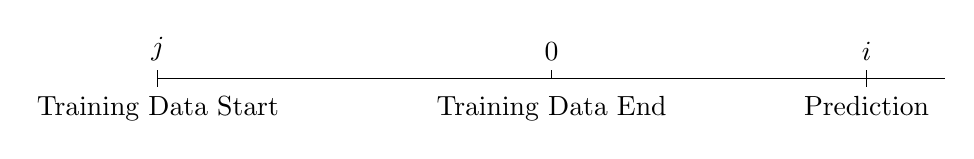
\begin{tikzpicture}[snake=zigzag, line before snake = 5mm, line after snake = 5mm]
    % draw horizontal line   
    \draw (0,0) -- (10,0);

    \draw (0cm, 3pt) -- (0cm, -3pt);
    \draw (5cm, 3pt) -- (5cm, 0pt);
    \draw (9cm, 3pt) -- (9cm, -3pt);
    

    % draw nodes
    \draw (0,0) node[below=3pt] {Training Data Start} node[above=3pt] {$j$};

    \draw (5,0) node[below=3pt] {Training Data End} node[above=3pt] {0};
    \draw (6,0) node[below=3pt] {$  $} node[above=3pt] {$  $};
    \draw (9,0) node[below=3pt] {Prediction} node[above=3pt] {$i$};
  \end{tikzpicture}




\end{document}